% Unit 106 English translation of chapter8.tex lines 1--174.
% Source: Methods of Algebra, Volume 2, commit
% 9a5803ff77dd3257484cb177f851a73770a59dd3 (CC BY 4.0).
% stable-unit-id: o014.aljabr2.chapter8.simplicial-objects
% Coverage: the opening of Chapter 8 and complete Section 8.1;
% stops immediately before Section 8.2 at line 175.

% Original source: Copyright 2024 Wen-Wei Li, CC BY 4.0.

% segment-id: o014.li2.chapter8.simplicial-objects.h001
\chapter{Simplicial Methods}\label{sec:simplicial}
\hypertarget{o014.aljabr2.chapter8.simplicial-objects}{ }
% segment-id: o014.li2.chapter8.simplicial-objects.p001
Let $\simpDelta$ be the category of nonempty finite ordinals. By definition,
a simplicial object in a category $\mathcal{C}$ is a functor
$X:\simpDelta^{\opp}\to\mathcal{C}$. Equivalently, it can be described as a
sequence of objects $X_0,X_1,\ldots$ together with morphisms
$d_i:X_n\to X_{n-1}$ (faces) and $s_j:X_n\to X_{n+1}$ (degeneracies), for
$0\leq i,j\leq n$, satisfying the family of identities
\eqref{eqn:simplicial-identity}. Such functors form the category
$\cate{s}\mathcal{C}$. In the special case $\mathcal{C}=\cate{Set}$, these
objects are also called simplicial sets. Their basic theory is discussed in
\S\S\ref{sec:simplicial-method}--\ref{sec:simplicial-set}. Write
$\cate{FinOrd}$ for the category of finite ordinals. If the functor underlying
a simplicial object $X$ extends to a functor
$\cate{FinOrd}\to\mathcal{C}$, then $X$ is called an augmented simplicial
object. This is equivalent to adding a term $X_{-1}$ in degree $-1$ to the
data $(X_n,d_i,s_j)_{n,i,j}$.

% segment-id: o014.li2.chapter8.simplicial-objects.p002
Simplicial sets originate in topology. The basic idea is to decompose a space
as a gluing of simplices; the intuitive picture of simplices (a point, a line
segment, a triangle, a tetrahedron, and so forth) is
% segment-id: o014.li2.chapter8.simplicial-objects.g001
\begin{center}\begin{tabular}{ccccc}
	$0$ dimensions & $1$ dimension & $2$ dimensions & $3$ dimensions & $\cdots$ \\
	
\begin{tikzpicture}[baseline=(P)] \fill[black] (0.5, 0.5) circle[radius=0.07]; \coordinate (P) at (0, 0.5); \end{tikzpicture} &
	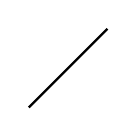
\begin{tikzpicture}[baseline=(P)] \draw[thick] (0,0) -- (1,1); \coordinate (P) at (0.5, 0.5); \end{tikzpicture} &
	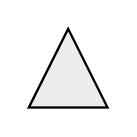
\begin{tikzpicture}[baseline=(P)] \filldraw[thick, fill=gray!15] (0,1) -- (-0.5, 0) -- (0.5, 0) --cycle; \coordinate (P) at (0, 0.5); \end{tikzpicture} &
	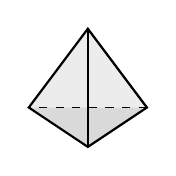
\begin{tikzpicture}[baseline=(P)]
		\fill[color=gray!15] (0, 1) -- (0.75, 0) -- (0, -0.5) -- (-0.75, 0) --cycle;
		\fill[color=gray!30] (0.75, 0) -- (0, -0.5) -- (-0.75, 0) --cycle;
		\draw[dashed] (0.75, 0) -- (-0.75, 0);
		\draw[thick] (0, 1) -- (0.75, 0) -- (0, -0.5) -- (-0.75, 0) --cycle;
		\draw[thick] (0, 1) -- (0, -0.5);
		\coordinate (P) at (0, 0.3);
	\end{tikzpicture} &
	$\cdots$
\end{tabular}\end{center}
Such a decomposition gives a concrete, combinatorial way to understand
homology, homotopy, and other questions about spaces. The rigorous
formulation used here was introduced by S.\ Eilenberg and J.\ A.\ Zilber in
1950. The language of simplicial sets has a broad reach and is not confined
to classical topological questions. For example, it can describe a category
through the construction called its ``nerve'', introduced in
\S\ref{sec:nerves}. Category theory concerns objects in diagrams (shown as
zero-dimensional points), morphisms (shown as one-dimensional arrows), and
commutativity (associated with two-dimensional pieces such as triangles or
squares). It is therefore unsurprising that categories and spaces can be
united within the same mathematical structure.

% segment-id: o014.li2.chapter8.simplicial-objects.p003
After introducing nerves and classifying spaces as basic examples of
simplicial sets, \S\ref{sec:geom-realization} returns to the geometric
intuition and defines the geometric realization $|X|$ of a simplicial set
$X$. Theorem~\ref{prop:geom-Sing-adjunction} shows that geometric realization
and the singular-set functor $\mathrm{Sing}$ familiar from topology form an
adjoint pair
% segment-id: o014.li2.chapter8.simplicial-objects.q001
\[\begin{tikzcd}
	{|\cdot|}: \cate{sSet} \arrow[shift left, r] & \cate{Top} : \mathrm{Sing}. \arrow[shift left, l]
\end{tikzcd}\]
If $\cate{Top}$ is replaced by the category $\cate{CGHaus}$ of compactly
generated Hausdorff spaces, customary in homotopy theory, geometric
realization also satisfies $|X\times Y|\simeq|X|\times|Y|$. The product on
the left is formed degreewise from the two simplicial sets. The proof is
related to triangulating products and involves some nontrivial combinatorial
details; since this is not a topology textbook, we shall not pursue them.

% segment-id: o014.li2.chapter8.simplicial-objects.p004
For the subject of this book, simplicial objects in an abelian category
$\mathcal{A}$ are more important. In this situation,
$\cate{s}\mathcal{A}$ is also an abelian category; for example, simplicial
abelian groups form the abelian category $\cate{sAb}$. The fundamental result
is the Dold--Kan correspondence in \S\ref{sec:Dold-Kan}
(Theorem~\ref{prop:Dold-Kan}), which, for an abelian category $\mathcal{A}$,
gives an adjoint pair of equivalences
% segment-id: o014.li2.chapter8.simplicial-objects.q002
\[\begin{tikzcd}
	\Gamma: \cate{s}\mathcal{A} \arrow[shift left, r] & \cate{Ch}_{\geq 0}(\mathcal{A}): \mathrm{N}, \arrow[shift left, l]
\end{tikzcd}\]
where $\cate{Ch}_{\geq0}(\mathcal{A})$ denotes the abelian category of
nonnegatively graded chain complexes over $\mathcal{A}$. The functor
$\mathrm{N}$ maps a simplicial object $X$ to the corresponding normalized
chain complex $\mathrm{N}X$. More precisely, define the unnormalized chain
complex of $X\in\Obj(\cate{s}\mathcal{A})$ by
% segment-id: o014.li2.chapter8.simplicial-objects.q003
\[ \mathrm{C}X := \left( X_n, \partial_n\right)_{n \geq 0}, \quad \partial_n := \sum_{i=0}^n (-1)^i d_i : X_n \to X_{n-1}. \]
Then $\mathrm{N}X$ may be taken as the chain subcomplex of $\mathrm{C}X$
given by $(\mathrm{N}X)_n:=\bigcap_{i=1}^n\Ker(d_i)$, or regarded as the
quotient of $\mathrm{C}X$ by its degenerate part. The isomorphism between
these two forms is the content of Proposition~\ref{prop:Dold-Kan-v}.
Moreover, Theorem~\ref{prop:Dold-Kan-N-C} shows that the inclusion morphism
$u:\mathrm{N}X\to\mathrm{C}X$ is a quasi-isomorphism of chain complexes.

% segment-id: o014.li2.chapter8.simplicial-objects.p005
The Dold--Kan correspondence makes simplicial theory one of the sources of
homological algebra, not only historically but also conceptually and
technically. Simplicial methods can explain and enrich the basic operations
on complexes or chain complexes; for example, homotopy and contractibility
have simplicial versions and thereby acquire topological interpretations.
This is discussed in \S\ref{sec:homology-computation}.

% segment-id: o014.li2.chapter8.simplicial-objects.p006
Another application connects simplicial methods with the theory of monads
from \S\ref{sec:Beck}. In this way, an object of a category can be canonically
expanded into an augmented simplicial object or an augmented cosimplicial
object. Because these techniques are related to the operation of ``adding a
bar'' in Hochschild homology, they are collectively called bar constructions
and form the subject of \S\ref{sec:bar-resolution}. Through the Dold--Kan
correspondence and some observations about contractibility, bar constructions
explain the standard resolutions in Hochschild theory (see \S\ref{sec:HH})
and group cohomology (see \S\ref{sec:G-mod}); they all turn out to arise from
a single idea at a higher level. The Exercises contain another extension of
the bar construction.

% segment-id: o014.li2.chapter8.simplicial-objects.p007
By definition, the bisimplicial objects discussed in
\S\ref{sec:bisimplicial} are simply functors
$\simpDelta^{\opp}\times\simpDelta^{\opp}\to\mathcal{C}$; they form the
category $\cate{s}^2\mathcal{C}$. If $\mathcal{A}$ is an abelian category,
the Eilenberg--Zilber Theorem~\ref{prop:Eilenberg-Zilber}, which directly
concerns $\cate{s}^2\mathcal{A}$, is a fundamental construction in algebraic
topology. From the viewpoint of pure category theory, if $\mathcal{A}$ is a
monoidal category (for example, $\mathcal{A}=\cate{Ab}$), the theorem gives
two canonical monoidal structures, in opposite directions, on the functor
$\mathrm{N}:\cate{s}\mathcal{A}\to\cate{Ch}_{\geq0}(\mathcal{A})$. The
applications of bisimplicial objects are not limited to this, however.

% segment-id: o014.li2.chapter8.simplicial-objects.p008
The last two sections of this chapter, \S\ref{sec:closed-simplicial} and
\S\ref{sec:mapping-cone-revisited}, discuss $\Hom$ objects and mapping cones
for simplicial sets, respectively. On the one hand, they correspond to
mapping spaces and cones in the topological intuition. On the other hand, in
the case of abelian groups, the Dold--Kan correspondence gives the familiar
$\Hom$ chain complexes and mapping cones. Thus the related constructions on
complexes or chain complexes receive a transparent explanation, while for
topologists all of this is already familiar.

% segment-id: o014.li2.chapter8.simplicial-objects.n001
\begin{wenxintishi}
	Sections \S\S\ref{sec:simplicial-method}--\ref{sec:geom-realization} form
	the backbone of the simplicial methods in this chapter;
	\S\S\ref{sec:Dold-Kan}--\ref{sec:bar-resolution} are directly connected
	with chain complexes; and although
	\S\S\ref{sec:bisimplicial}--\ref{sec:mapping-cone-revisited} accord with
	the contents of the preceding books, these sections are more advanced.
	Unlike the material of the other chapters, simplicial methods are not
	logically necessary. Their ideas and techniques are nevertheless part of a
	mathematician's basic toolkit and provide a foundation for entering higher
	algebra. Some arguments about simplicial objects occasionally involve
	lengthy routine verifications (as in \S\ref{sec:Dold-Kan}); this is a
	consequence of the definitions, and readers may decide for themselves how
	far they wish to follow such details.
\end{wenxintishi}

% segment-id: o014.li2.chapter8.simplicial-objects.h002
\section{Simplicial Objects}\label{sec:simplicial-method}
% segment-id: o014.li2.chapter8.simplicial-objects.p009
In Remark~\ref{rem:walking-algebra}, we recalled monotone maps between
partially ordered sets and used them to define the category $\cate{FinOrd}$
of finite ordinals. This chapter focuses on its full subcategory
$\simpDelta$ consisting of the nonempty ordinals.

% segment-id: o014.li2.chapter8.simplicial-objects.d001
\begin{definition}
	\index[sym1]{Delta-simp@$\simpDelta$}
	\index[sym1]{[n]}
	Let $\simpDelta$ be the category of all nonempty finite ordinals and
	monotone maps between them. In other words, its objects are the totally
	ordered sets $[n]:=\{0,\ldots,n\}$ for $n\in\Z_{\geq0}$, and its morphisms
	are monotone maps.
\end{definition}

% segment-id: o014.li2.chapter8.simplicial-objects.p010
Note that $[n]$ should not be confused with $\mathbf{n}$, which in this book
denotes the totally ordered set $\{0,\ldots,n-1\}$ or the corresponding
category.

% segment-id: o014.li2.chapter8.simplicial-objects.p011
Every morphism $[l]\to[n]$ in $\simpDelta$ has a unique factorization as a
surjective monotone map followed by an injective monotone map,
% segment-id: o014.li2.chapter8.simplicial-objects.q004
\[ [l] \twoheadrightarrow [m] \hookrightarrow [n], \quad n \geq m \leq l. \]
An injective (respectively, surjective) map of this kind can be decomposed
further into pieces that at each step omit exactly one element (respectively,
identify exactly two elements). In other words, every morphism can be
factored as a composite of the following two kinds of morphisms.
% segment-id: o014.li2.chapter8.simplicial-objects.q005
\begin{center}\begin{tabular}{|l|p{0.74\textwidth}|} \hline
	Coface & $\mathrm{d}^i=\mathrm{d}^{n,i}:[n-1]\hookrightarrow[n]$, where
	$0\leq i\leq n$; the monotone injection omits only $i\in[n]$. \\ \hline
	Codegeneracy & $\mathrm{s}^j=\mathrm{s}^{n,j}:[n+1]\twoheadrightarrow[n]$,
	where $0\leq j\leq n$; the monotone surjection takes the value $j\in[n]$
	twice. \\ \hline
\end{tabular}\end{center}

% segment-id: o014.li2.chapter8.simplicial-objects.p012
An injective (respectively, surjective) monotone map can be decomposed into
cofaces (respectively, codegeneracies) in several ways, depending on the
order in which the elements are omitted (respectively, identified). The
following \emph{cosimplicial identities} are easy to verify:
% segment-id: o014.li2.chapter8.simplicial-objects.q006
\begin{equation}\label{eqn:cosimplicial-identity}\begin{array}{ll}
	\mathrm{d}^j \mathrm{d}^i = \mathrm{d}^i \mathrm{d}^{j-1}, & i < j, \\
	\mathrm{s}^j \mathrm{d}^i = \mathrm{d}^i \mathrm{s}^{j-1} & i < j, \\
	\mathrm{s}^j \mathrm{d}^j = \identity = \mathrm{s}^j \mathrm{d}^{j+1}, & \forall j, \\
	\mathrm{s}^j \mathrm{d}^i = \mathrm{d}^{i-1} \mathrm{s}^j, & i > j+1, \\
	\mathrm{s}^j \mathrm{s}^i = \mathrm{s}^i \mathrm{s}^{j+1}, & i \leq j.
\end{array}\end{equation}

% segment-id: o014.li2.chapter8.simplicial-objects.p013
Examining how one passes between the various decompositions of an injective
(respectively, surjective) monotone map shows that the cofaces,
codegeneracies, and \eqref{eqn:cosimplicial-identity} give a complete system
of generators and relations for the morphisms of $\simpDelta$.

% segment-id: o014.li2.chapter8.simplicial-objects.p014
Viewed in $\simpDelta^{\opp}$, these give the corresponding morphisms
% segment-id: o014.li2.chapter8.simplicial-objects.q007
\begin{center}\begin{tabular}{|l|l|l|} \hline
		Face & $\mathrm{d}_i = \mathrm{d}^n_i: [n] \xrightarrow{\opp} [n-1]$ & $0 \leq i \leq n$ \\ \hline
		Degeneracy & $\mathrm{s}_j = \mathrm{s}^n_j: [n] \xrightarrow{\opp} [n+1]$ & $0 \leq j \leq n$ \\ \hline
\end{tabular}\end{center}
The symbol $\xrightarrow{\opp}$ merely reminds us that the arrow lies in the
opposite category $\simpDelta^{\opp}$. Reversing
\eqref{eqn:cosimplicial-identity} gives the \emph{simplicial identities}
% segment-id: o014.li2.chapter8.simplicial-objects.q008
\begin{equation}\label{eqn:simplicial-identity}\begin{array}{ll}
	\mathrm{d}_i \mathrm{d}_j = \mathrm{d}_{j-1} \mathrm{d}_i, & i < j \\
	\mathrm{d}_i \mathrm{s}_j = \mathrm{s}_{j-1} \mathrm{d}_i & i < j \\
	\mathrm{d}_j \mathrm{s}_j = \identity = \mathrm{d}_{j+1} \mathrm{s}_j, & \forall j \\
	\mathrm{d}_i \mathrm{s}_j  = \mathrm{s}_j \mathrm{d}_{i-1}, & i > j+1 \\
	\mathrm{s}_i \mathrm{s}_j = \mathrm{s}_{j+1} \mathrm{s}_i, & i \leq j.
\end{array}\end{equation}
\index{simplicial identities}

% segment-id: o014.li2.chapter8.simplicial-objects.d002
\begin{definition}\label{def:simplicial-obj}
	\index{simplicial object}
	\index{cosimplicial object}
	\index{simplicial object!augmented}
	\index[sym1]{sC@$\cate{s}\mathcal{C}, \cate{cs}\mathcal{C}$}
	For a category $\mathcal{C}$,
	\begin{itemize}
		\item a \emph{simplicial object} in it means a functor
		$\simpDelta^{\opp}\to\mathcal{C}$; all simplicial objects form the
		category
		$\cate{s}\mathcal{C}:=\mathcal{C}^{\simpDelta^{\opp}}$;
		\item a \emph{cosimplicial object} in it means a functor
		$\simpDelta\to\mathcal{C}$; all cosimplicial objects form the category
		$\cate{cs}\mathcal{C}:=\mathcal{C}^{\simpDelta}$.
	\end{itemize}

	Consequently,
	$(\cate{cs}\mathcal{C})^{\opp}\simeq\cate{s}(\mathcal{C}^{\opp})$.
	If the functor underlying a simplicial (respectively, cosimplicial) object
	has an extension to $\cate{FinOrd}^{\opp}$ (respectively,
	$\cate{FinOrd}$), then the object is called \emph{augmented}.
\end{definition}

\index[sym1]{di@$d_i, \mathrm{d}_i$}
\index[sym1]{sj@$s_j, \mathrm{s}_j$}
% segment-id: o014.li2.chapter8.simplicial-objects.p015
By the preceding discussion, giving a simplicial object $X$ is equivalent to
giving a family of objects $(X_n)_{n\geq0}$ in $\mathcal{C}$ together with a
family of morphisms satisfying \eqref{eqn:simplicial-identity},
% segment-id: o014.li2.chapter8.simplicial-objects.q009
\[ d_i = d^n_i: X_n \to X_{n-1} \; \text{(face)}, \quad s_j = s^n_j: X_n \to X_{n+1} \; \text{(degeneracy)}, \quad 0 \leq i, j \leq n. \]
The object $X_n$ is called the degree-$n$ term of $X$. A morphism from a
simplicial object $X$ to $Y$ is equivalently a family of morphisms
$(f_n:X_n\to Y_n)_{n\geq0}$ in $\mathcal{C}$ satisfying, for every $n\geq0$,
the compatibility conditions
% segment-id: o014.li2.chapter8.simplicial-objects.q010
\[ d^{n+1}_i f_{n+1} = f_n d^{n+1}_i, \quad s^n_j f_n = f_{n+1} s^n_j . \]

% segment-id: o014.li2.chapter8.simplicial-objects.p016
Dually, giving a cosimplicial object $X$ is equivalent to giving a family of
objects $(X^n)_{n\geq0}$ in $\mathcal{C}$ together with a family of morphisms
satisfying \eqref{eqn:cosimplicial-identity},
% segment-id: o014.li2.chapter8.simplicial-objects.q011
\[ d^i = d^{n, i}: X^{n-1} \to X^n \; \text{(coface)}, \quad s^j = s^{n, j}: X^{n+1} \to X^n \; \text{(codegeneracy)}, \quad 0 \leq i, j \leq n. \]
Its morphisms are families of morphisms $f^n:X^n\to Y^n$ compatible with
all $d^i$ and $s^j$.

% segment-id: o014.li2.chapter8.simplicial-objects.p017
An augmentation of a simplicial (respectively, cosimplicial) object $X$ is
equivalently the addition to the data of a morphism $X_0\to X_{-1}$
(respectively, $X^{-1}\to X^0$) and a commutative diagram
% segment-id: o014.li2.chapter8.simplicial-objects.q012
$\begin{tikzcd}
	X_1 \arrow[shift left, r, "d_0"] \arrow[shift right, r, "d_1"'] & X_0 \arrow[r, "\epsilon"] & X_{-1}
\end{tikzcd}$
(respectively, its dual). This morphism is called the augmentation morphism.

% segment-id: o014.li2.chapter8.simplicial-objects.cv001
\begin{convention}
	For a morphism $\phi:[m]\to[n]$ in $\simpDelta$ and a simplicial
	(respectively, cosimplicial) object $X$ in a category $\mathcal{C}$, denote
	the corresponding morphism by $\phi^*:X_n\to X_m$ (respectively,
	$\phi_*:X^m\to X^n$).
\end{convention}

% segment-id: o014.li2.chapter8.simplicial-objects.r001
\begin{remark}\label{rem:semisimplicial}
	\index{semisimplicial object}
	All nonempty ordinals and the injective monotone maps between them form a
	category $\simpDelta_+$. A functor of the form
	$\simpDelta_+^{\opp}\to\mathcal{C}$ is called a \emph{semisimplicial
	object} in $\mathcal{C}$. This is equivalent to deleting the degeneracy
	morphisms $s_j$ and the associated conditions from the definition of a
	simplicial object. Every simplicial object gives a corresponding
	semisimplicial object. Augmented semisimplicial objects may be defined
	similarly. The case of cosemisimplicial objects is entirely dual.
\end{remark}

% segment-id: o014.li2.chapter8.simplicial-objects.eg001
\begin{example}\label{eg:const-simplicial}
	\index{simplicial object!constant}
	Let $C\in\Obj(\mathcal{C})$. The corresponding \emph{constant simplicial
	object} $\mathrm{const}(C)$ is determined by
	$\mathrm{const}(C)_n=C$ and $s_j=\identity_C=d_i$ for all $n,i,j$. As a
	simple exercise, check that
	% segment-id: o014.li2.chapter8.simplicial-objects.q013
	\[ \left\{ \text{augmentations of }X\right\} \xleftrightarrow{1:1} \left\{ (C, \varphi): C \in \Obj(\mathcal{C}), \; \varphi: X \to \mathrm{const}(C)  \right\}. \]
	Concretely, for a given augmentation of $X$, take $C=X_{-1}$ and let
	$\varphi_n$ be the composite
	$X_n\xrightarrow{\iota_k^*}X_0\to X_{-1}$, where
	$\iota_k:[0]\to[n]$ sends $0$ to any $k$ with
	$0\leq k\leq n$. The case of constant cosimplicial objects is entirely
	similar.
\end{example}

% segment-id: o014.li2.chapter8.simplicial-objects.eg002
\begin{example}
	Let $B\to A$ be a morphism in a category $\mathcal{C}$. If the following
	fiber products exist,
	% segment-id: o014.li2.chapter8.simplicial-objects.q014
	\[ X_n := \underbracket{B \dtimes{A} \cdots \dtimes{A} B}_{n+1 \;\text{factors}}, \quad n \geq 0, \]
	each morphism $f:[m]\to[n]$ induces a morphism $X_n\to X_m$ whose $i$th
	component is the projection
	$B\dtimes{A}\cdots\dtimes{A}B\xrightarrow{\mathrm{pr}_{f(i)}}B$. This
	gives a simplicial object $X$ in $\mathcal{C}$. It is augmented by taking
	$B\to A$ as the morphism $X_0\to X_{-1}$.
\end{example}

% segment-id: o014.li2.chapter8.simplicial-objects.r002
\begin{remark}[Order-reversal duality]\label{rem:simpDelta-order-reversal}
	For each $n\in\Z_{\geq0}$, define a bijection $w_n$ of
	$\{0,\ldots,n\}$ with itself by $w_n(i)=n-i$. Define an autoisomorphism
	$w$ of the category $\simpDelta$ that preserves the objects $[n]$ and maps
	a morphism $f:[n]\to[m]$ to $wf:=w_mfw_n$. Note that
	% segment-id: o014.li2.chapter8.simplicial-objects.q015
	\[ w^2 = \identity_{\simpDelta}, \quad w \mathrm{d}^{n, i} = \mathrm{d}^{n, n-i}, \quad w \mathrm{s}^{n, j} = \mathrm{s}^{n, n-j}. \]
	A more intrinsic viewpoint is that $w$ maps $[n]$ to the poset with the
	reversed order $[n]^{\opp}$, or, when regarded as a category, to its
	opposite category. This category is still uniquely isomorphic to $[n]$.
	The action of $w$ on morphisms is expressed by the commutative diagram
	% segment-id: o014.li2.chapter8.simplicial-objects.q016
	\[\begin{tikzcd}
		{[m]^{\opp}} \arrow[r, "{f^{\opp}}", "\text{monotone}"'] & {[n]^{\opp}} \\
		{[m]} \arrow[r, "\text{monotone}", "{wf}"'] \arrow[u, "\sim" sloped] & {[n]} \arrow[u, "\sim" sloped]
	\end{tikzcd} \quad f^{\opp} \xlongequal{\text{as a map}} f. \]
	For every category $\mathcal{C}$, this gives an autoisomorphism
	$X\mapsto X\circ w$ of $\cate{s}\mathcal{C}$ (respectively,
	$\cate{cs}\mathcal{C}$).
\end{remark}

% segment-id: o014.li2.chapter8.simplicial-objects.p018
Finally, we outline the relation between monoidal structures and simplicial
objects.

% segment-id: o014.li2.chapter8.simplicial-objects.d003
\begin{definition}\label{def:monoidal-sObj}
	Every functor $F:\mathcal{C}\to\mathcal{D}$ induces a functor
	$\cate{s}\mathcal{C}\to\cate{s}\mathcal{D}$ that maps the data
	$(X_n,d_i,s_j)_{n,i,j}$ to $(FX_n,Fd_i,Fs_j)_{n,i,j}$. Moreover, there is
	a direct relation
	$\cate{s}(\mathcal{C}_1\times\mathcal{C}_2)\simeq
	\cate{s}\mathcal{C}_1\times\cate{s}\mathcal{C}_2$.

	Apply this observation to a monoidal category $\mathcal{C}$ and the
	bifunctor $\otimes:\mathcal{C}\times\mathcal{C}\to\mathcal{C}$. For
	every $X,Y\in\Obj(\cate{s}\mathcal{C})$, define
	$X\otimes Y\in\Obj(\cate{s}\mathcal{C})$ so that its degree-$n$ term is
	$X_n\otimes Y_n$, while its face and degeneracy morphisms have the forms
	$d_i\otimes d_i$ and $s_j\otimes s_j$, respectively.
\end{definition}

% segment-id: o014.li2.chapter8.simplicial-objects.p019
Thus, if $\mathcal{C}$ is a monoidal category, then
$\cate{s}\mathcal{C}$ also has a corresponding monoidal structure, with the
constant simplicial object $\mathrm{const}(\munit)$ as its unit. The analogous
statement holds for cosimplicial objects.
